\documentclass{sigchi}

% Arabic page numbers for submission.  Remove this line to eliminate
% page numbers for the camera ready copy
% \pagenumbering{arabic}

% Load basic packages
\usepackage{balance}       % to better equalize the last page
\usepackage{graphics}      % for EPS, load graphicx instead
\usepackage[T1]{fontenc}   % for umlauts and other diaeresis
\usepackage{txfonts}
\usepackage{mathptmx}
\usepackage[pdflang={en-US},pdftex]{hyperref}
\usepackage{color}
\usepackage{booktabs}
\usepackage{textcomp}

% Some optional stuff you might like/need.
\usepackage{microtype}        % Improved Tracking and Kerning
% \usepackage[all]{hypcap}    % Fixes bug in hyperref caption linking
\usepackage{ccicons}          % Cite your images correctly!
% \usepackage[utf8]{inputenc} % for a UTF8 editor only

% If you want to use todo notes, marginpars etc. during creation of
% your draft document, you have to enable the "chi_draft" option for
% the document class. To do this, change the very first line to:
% "\documentclass[chi_draft]{sigchi}". You can then place todo notes
% by using the "\todo{...}"  command. Make sure to disable the draft
% option again before submitting your final document.
\usepackage{todonotes}

% Paper metadata (use plain text, for PDF inclusion and later
% re-using, if desired).  Use \emtpyauthor when submitting for review
% so you remain anonymous.
\def\plaintitle{Wikipedia's Edit Filters}
\def\plainauthor{First Author, Second Author, Third Author,
  Fourth Author, Fifth Author, Sixth Author}
\def\emptyauthor{}
\def\plainkeywords{Authors' choice; of terms; separated; by
  semicolons; include commas, within terms only; required.}
\def\plaingeneralterms{Documentation, Standardization}

% llt: Define a global style for URLs, rather that the default one
\makeatletter
\def\url@leostyle{%
  \@ifundefined{selectfont}{
    \def\UrlFont{\sf}
  }{
    \def\UrlFont{\small\bf\ttfamily}
  }}
\makeatother
\urlstyle{leo}

% To make various LaTeX processors do the right thing with page size.
\def\pprw{8.5in}
\def\pprh{11in}
\special{papersize=\pprw,\pprh}
\setlength{\paperwidth}{\pprw}
\setlength{\paperheight}{\pprh}
\setlength{\pdfpagewidth}{\pprw}
\setlength{\pdfpageheight}{\pprh}

% Make sure hyperref comes last of your loaded packages, to give it a
% fighting chance of not being over-written, since its job is to
% redefine many LaTeX commands.
\definecolor{linkColor}{RGB}{6,125,233}
\hypersetup{%
  pdftitle={\plaintitle},
% Use \plainauthor for final version.
%  pdfauthor={\plainauthor},
  pdfauthor={\emptyauthor},
  pdfkeywords={\plainkeywords},
  pdfdisplaydoctitle=true, % For Accessibility
  bookmarksnumbered,
  pdfstartview={FitH},
  colorlinks,
  citecolor=black,
  filecolor=black,
  linkcolor=black,
  urlcolor=linkColor,
  breaklinks=true,
  hypertexnames=false
}

% create a shortcut to typeset table headings
% \newcommand\tabhead[1]{\small\textbf{#1}}

% End of preamble. Here it comes the document.
\begin{document}

\title{\plaintitle}

\numberofauthors{3}
\author{%
  \alignauthor{Leave Authors Anonymous\\
    \affaddr{for Submission}\\
    \affaddr{City, Country}\\
    \email{e-mail address}}\\
  \alignauthor{Leave Authors Anonymous\\
    \affaddr{for Submission}\\
    \affaddr{City, Country}\\
    \email{e-mail address}}\\
  \alignauthor{Leave Authors Anonymous\\
    \affaddr{for Submission}\\
    \affaddr{City, Country}\\
    \email{e-mail address}}\\
}

\maketitle

\begin{abstract}
  Abstracts should be about 150 words and
  are required.
\end{abstract}

\category{H.5.m.}{Information Interfaces and Presentation
  (e.g. HCI)}{Miscellaneous} \category{See
  \url{http://acm.org/about/class/1998/} for the full list of ACM
  classifiers. This section is required.}{}{}

\keywords{\plainkeywords}

\section{Introduction}

There's an inscription in Code 2.0:
"Code 2.0
TO WIKIPEDIA, THE ONE SURPRISE THAT TEACHES MORE THAN EVERYTHING HERE." (p.v)~\cite{Lessig2006}

\section{Genesis}

% When and why were Wikipedia edit filters introduced?

Edit filters were first introduced on the English Wikipedia in 2009 under the name ``abuse filters''.
Their clear purpose was to cope with the rising(syn) amount of vandalism as well as ``common newbie mistakes'' the encyclopedia faced~\cite{Signpost2009}.

% TODO: when and why was the extension renamed

%************************************************************************

\section{Intended Contributions}
%Epistemological interest

What do we want to know?

Core questions:

We wanted to improve our understanding of the role of filters in existing algorithmic quality-control mechanisms (bots, ORES, humans).

Which type of tasks do these filters take over in comparison to the other mechanisms? How these tasks evolve over time (are they changes in the type, number, etc.)?

Since filters are classical rule-based systems, what are suitable areas of application for such rule-based system in contrast to the other ML-based approaches.


\begin{itemize}
    \item Description of how filters integrate into the algorithmic quality control mechanism in Wikipedia
    \item Do filters work the desired way/help for a smoother Wikipedia service or is it a lot of work to maintain them and the usefulness is questionable?
    \item What can we filter with a REGEX? And what not? Are regexes the suitable technology for the means the community is trying to achieve?
    \item Filter are classical rule-based systems. What are suitable areas of application for such rule-based system in contrast to ML systems?
\end{itemize}


What can we study?

\begin{itemize}
    \item Discussions on filter patterns? On filter repercussions?
    \item Whether filters work the desired way/help for a smoother Wikipedia service or is it a lot of work to maintain them and the usefullness is questionable?
    \item What can we filter with a REGEX? And what not? Are regexes the suitable technology for the means the community is trying to achieve?
    \item add also "af\_enabled" column to filter list; could be that the high hit count was made by false positives, which will have led to disabling the filter (TODO: that's a very interesting question actually; how do we know the high number of hits were actually leggit problems the filter wanted to catch and no false positives?)
\end{itemize}


\begin{comment}
* Think about: what's the computer science take on the field? How can we design a "better"/more efficient/more user friendly system? A system that reflects particular values (vgl Code 2.0, Chapter 3, p.34)?
  * go over notes in the filter classification and think about interesting controversies, things that attract the attention
  * what are useful categories
  * GT is good for tackling controversial questions: e.g. are filters with disallow action a too severe interference with the editing process that has way too much negative consequences? (e.g. driving away new comers?)

* What can we study?
  * Question: Is it worth it to use a filter which has many side effects?
  * Do filters work the desired way/help for a smoother Wikipedia service or is it a lot of work to maintain them and the usefulness is questionable?
  * Precision/Recall: False Positives? were filters shut down, bc they matched more False positives than they had real value?
  * How has the notion of vandalism changed over time (not particularly computer sciency..)?
  * What are disallow/block filters doing? Is it too great an intervention that drives new editors away? (Can we answer that?)
  * Is it worth it to use a filter which has many side effects?
  * What are discussions on filter patterns? On filter repercussions?
  * What can we filter with a REGEX? And what not? Are regexes the suitable technology for the means the community is trying to achieve?
  * GT is good for tackling controversial questions: e.g. are filters with disallow action a too severe interference with the editing process that has way too much negative consequences? (e.g. driving away new comers?)

## TODO

* How can we improve it from a computer scientist's/engineer's perspective?
* What task do the edit filters try to solve? Why does this task exist?/Why is it important?
* Why are there mechanisms triggered befor an edit gets published (such as edit filters), and such triggered afterwards (such as bots)? Is there a qualitative difference?
* I want to help people to do their work better using a technical system (e.g. the edit filters). How can I do this?
* The edit filter system can be embedded in the vandalism prevention frame. Are there other contexts/frames for which it is relevant?
\end{comment}

%************************************************************************

\section{Algorithmic quality-control mechanisms on Wikipedia}
%Context
Context of work: algorithmic quality-control mechanisms (bots, ORES, humans) → filter?

%TODO Literature review!
Distinction filters/Bots: what tasks are handled by bots and what by filters (and why)? What difference does it make for admins? For users whose edits are being targeted?

\subsection{Vandalism on Wikipedia}

Edit filters were initially introduced as a vandalism prevention mechanism (one of several).
The aim of this section is to provide a better understanding of vandalism on Wikipedia. (What is vandalism, and what not; who engages in vandalism; who is striving to prevent it and with what means)

\url{https://en.wikipedia.org/wiki/Wikipedia:Vandalism}

"This is not a noticeboard for vandalism. Report vandalism from specific users at Wikipedia:Administrator intervention against vandalism, or Wikipedia:Requests for page protection for specific pages.
Not to be confused with Wikipedia:Disruptive editing."

"This page documents an English Wikipedia policy."

"This page in a nutshell: Intentionally making abusive edits to Wikipedia will result in a block."

DEF Vandalism:
"On Wikipedia, vandalism has a very specific meaning: editing (or other behavior) deliberately intended to obstruct or defeat the project's purpose, which is to create a free encyclopedia, in a variety of languages, presenting the sum of all human knowledge."
"The malicious removal of encyclopedic content, or the changing of such content beyond all recognition, without any regard to our core content policies of neutral point of view (which does not mean no point of view), verifiability and no original research, is a deliberate attempt to damage Wikipedia. There, of course, exist more juvenile forms of vandalism, such as adding irrelevant obscenities or crude humor to a page, illegitimately blanking pages, and inserting obvious nonsense into a page. Abusive creation or usage of user accounts and IP addresses may also constitute vandalism."

Consequences of vandalism, vandalism management
"Vandalism is prohibited. While editors are encouraged to warn and educate vandals, warnings are by no means a prerequisite for blocking a vandal (although administrators usually only block when multiple warnings have been issued). "

"Even if misguided, willfully against consensus, or disruptive, any good-faith effort to improve the encyclopedia is not vandalism."
"For example, edit warring over how exactly to present encyclopedic content is not vandalism." !!!
"Careful consideration may be required to differentiate between edits that are beneficial, edits that are detrimental but well-intentioned, and edits that are vandalism."
"If it is clear that the editor in question is intending to improve Wikipedia, those edits are not vandalism, even if they violate some other core policy of Wikipedia."
"When editors are editing in good faith, mislabeling their edits as vandalism makes them less likely to respond to corrective advice or to engage collaboratively during a disagreement,"

Handling
"Upon discovering vandalism, revert such edits, using the undo function or an anti-vandalism tool. Once the vandalism is undone, warn the vandalizing editor. Notify administrators at the vandalism noticeboard of editors who continue to vandalize after multiple warnings, and administrators should intervene to preserve content and prevent further disruption by blocking such editors. Users whose main or sole purpose is clearly vandalism may be blocked indefinitely without warning."

"examples of suspicious edits are those performed by IP addresses, red linked, or obviously improvised usernames"

One of the strategies to spot vandalism is "Watching for edits tagged by the abuse filter. However, many tagged edits are legitimate, so they should not be blindly reverted. That is, do not revert without at least reading the edit."

"Warn the vandal. Access the vandal's talk page and warn them. A simple note explaining the problem with their editing is sufficient. If desired, a series of warning templates exist to simplify the process of warning users, but these templates are not required."

Types of vandalism \url{https://en.wikipedia.org/wiki/Wikipedia:Vandalism#Types_of_vandalism}:
  (Abuse of tags; Account creation, malicious; Avoidant vandalism; Blanking, illegitimate; Copyrighted material, repeated uploading of; Edit summary vandalism; Format vandalism; Gaming the system; Hidden vandalism; Hoaxing vandalism; Image vandalism; Link vandalism; Page creation, illegitimate; Page lengthening; Page-move vandalism; Silly vandalism; Sneaky vandalism; Spam external linking; Stockbroking vandalism; talk page vandalism; Template vandalism; User and user talk page vandalism; Vandalbots;)

\url{https://en.wikipedia.org/wiki/Wikipedia:Disruptive_editing}

"Disruptive editing is not vandalism, though vandalism is disruptive."
"Disruptive editing is not always intentional. Editors may be accidentally disruptive because they don't understand how to correctly edit, or because they lack the social skills or competence necessary to work collaboratively "
Okay what are disruptive edits that are not vandalism? (apart from edit wars)

"sometimes attracts people who seek to exploit the site as a platform for pushing a single point of view, original research, advocacy, or self-promotion."
"not verifiable through reliable sources or insisting on giving undue weight to a minority view."

"Collectively, disruptive editors harm Wikipedia by degrading its reliability as a reference source and by exhausting the patience of productive editors who may quit the project in frustration when a disruptive editor continues with impunity."

examples of disruptive editing:
"Engages in "disruptive cite-tagging"; adds unjustified {{citation needed}} tags to an article when the content tagged is already sourced, uses such tags to suggest that properly sourced article content is questionable."
"Rejects or ignores community input: resists moderation and/or requests for comment, continuing to edit in pursuit of a certain point despite an opposing consensus from impartial editors."

\subsection{Harassment and bullying}

%************************************************************************

\section{Methodology}

\subsection{Grounded Theory}
\subsection{Trace Ethnography}

\cite{GeiRib2011}
Introduce the methodology (and the concept) of trace ethnography.

Def
"combines the richness of participant-observation
with the wealth of data in logs so as to reconstruct
patterns and practices of users in distributed
sociotechnical systems."

"exploits the proliferation of
documents and documentary traces"

"traces not only
document events but are also used by participants
themselves to coordinate and render accountable many
activities"

"heterogeneous data – which include transaction logs,
version histories, institutional records, conversation
transcripts, and source code"
"allowing us to retroactively reconstruct specific actions
at a fine level of granularity"

"turn thin documentary traces into
“thick descriptions” [10] of actors and events"

"traces can only
be fully inverted through an ethnographic
understanding of the activities, people, systems, and
technologies which contribute to their production."

traditional ethnographic observation is costly and inpractical in distributed settings (and may miss phenomena that occur between sites)

Critique:
"it only can observe what the system
or platform records, which are always incomplete."

Concerns:
- ethical: breaching privacy via thickening the traces; no possibility for informed consent

\cite{GeiHal2017}
"when working with large-scale “found data” [36] of the traces
users leave behind when interacting on a platform, how do we best operationalize culturally-specific
concepts like conflict in a way that aligns with the particular context in which those traces were made?"

Star: "ethnography of infrastructure":
"discusses the “veridical” approach, in which “the information system
is taken unproblematically as a mirror of actions in the world, and often tacitly, as a complete
enough record of those actions” (p. 388).
She contrasts this with seeing the data as “a trace or record
of activities,” in which the information infrastructure “sits (often uneasily) somewhere between
research assistant to the investigator and found cultural artifact."

"Trace
ethnography is not “lurker ethnography” done by someone who never interviews or participates in
a community."
trace literacy --> get to know the community; know how to participate in it

thick description of different prototypical cases:

\subsection{Cooking Data With Care}
or Critical data science? Or both?

%************************************************************************

\section{Data}
%What is the best place herefor?

For the present analysis we have analysed EN Wikipedia's policies and guidelines on the one hand, and the database tables of the AbuseFilter extension on the other.

The \emph{abuse\_filter} and \emph{abuse\_filter\_action} tables from \emph{enwiki\_p} were downloaded on 6.01.2019 via quarry~\footnote{\url{https://quarry.wmflabs.org/}}.
The complete files can be found in the repository for the present paper~\cite{github}. % TODO add a more specific link

These tables, along with \emph{abuse\_filter\_log} and \emph{abuse\_filter\_history}, are created and used by the AbuseFilter MediaWiki extension~\cite{gerrit-abusefilter}.
Selected queries have been run against the \emph{abuse\_filter\_log} table as well.
Unfortunately, currently the \emph{abuse\_filter\_history} table is not exposed to the public due to security/privacy concerns~\cite{phabricator}.
We hope to be shortly able to access a view of this table in order to conduct historic inquirements.

The schemas of these tables can be viewed in Figures~\ref{fig:db-schemas-af},~\ref{fig:db-schemas-afl},~\ref{fig:db-schemas-afh} and~\ref{fig:db-schemas-afa}.

\begin{figure*}
\begin{verbatim}
abuse_filter
+--------------------+---------------------+------+-----+---------+----------------+
| Field              | Type                | Null | Key | Default | Extra          |
+--------------------+---------------------+------+-----+---------+----------------+
| af_id              | bigint(20) unsigned | NO   | PRI | NULL    | auto_increment |
| af_pattern         | blob                | NO   |     | NULL    |                |
| af_user            | bigint(20) unsigned | NO   | MUL | NULL    |                |
| af_user_text       | varbinary(255)      | NO   |     | NULL    |                |
| af_timestamp       | binary(14)          | NO   |     | NULL    |                |
| af_enabled         | tinyint(1)          | NO   |     | 1       |                |
| af_comments        | blob                | YES  |     | NULL    |                |
| af_public_comments | tinyblob            | YES  |     | NULL    |                |
| af_hidden          | tinyint(1)          | NO   |     | 0       |                |
| af_hit_count       | bigint(20)          | NO   |     | 0       |                |
| af_throttled       | tinyint(1)          | NO   |     | 0       |                |
| af_deleted         | tinyint(1)          | NO   |     | 0       |                |
| af_actions         | varbinary(255)      | NO   |     |         |                |
| af_global          | tinyint(1)          | NO   |     | 0       |                |
| af_group           | varbinary(64)       | NO   | MUL | default |                |
+--------------------+---------------------+------+-----+---------+----------------+
\end{verbatim}
  \caption{abuse\_filter schema}~\label{fig:db-schemas-af}
\end{figure*}

\begin{figure*}
\begin{verbatim}
abuse_filter_log
+------------------+---------------------+------+-----+---------+----------------+
| Field            | Type                | Null | Key | Default | Extra          |
+------------------+---------------------+------+-----+---------+----------------+
| afl_id           | bigint(20) unsigned | NO   | PRI | NULL    | auto_increment |
| afl_filter       | varbinary(64)       | NO   | MUL | NULL    |                |
| afl_user         | bigint(20) unsigned | NO   | MUL | NULL    |                |
| afl_user_text    | varbinary(255)      | NO   |     | NULL    |                |
| afl_ip           | varbinary(255)      | NO   | MUL | NULL    |                |
| afl_action       | varbinary(255)      | NO   |     | NULL    |                |
| afl_actions      | varbinary(255)      | NO   |     | NULL    |                |
| afl_var_dump     | blob                | NO   |     | NULL    |                |
| afl_timestamp    | binary(14)          | NO   | MUL | NULL    |                |
| afl_namespace    | tinyint(4)          | NO   | MUL | NULL    |                |
| afl_title        | varbinary(255)      | NO   |     | NULL    |                |
| afl_wiki         | varbinary(64)       | YES  | MUL | NULL    |                |
| afl_deleted      | tinyint(1)          | NO   |     | 0       |                |
| afl_patrolled_by | int(10) unsigned    | YES  |     | NULL    |                |
| afl_rev_id       | int(10) unsigned    | YES  | MUL | NULL    |                |
| afl_log_id       | int(10) unsigned    | YES  | MUL | NULL    |                |
+------------------+---------------------+------+-----+---------+----------------+
\end{verbatim}
  \caption{abuse\_filter\_log schema}~\label{fig:db-schemas-afl}
\end{figure*}

\begin{figure*}
\begin{verbatim}
abuse_filter_history
+---------------------+---------------------+------+-----+---------+----------------+
| Field               | Type                | Null | Key | Default | Extra          |
+---------------------+---------------------+------+-----+---------+----------------+
| afh_id              | bigint(20) unsigned | NO   | PRI | NULL    | auto_increment |
| afh_filter          | bigint(20) unsigned | NO   | MUL | NULL    |                |
| afh_user            | bigint(20) unsigned | NO   | MUL | NULL    |                |
| afh_user_text       | varbinary(255)      | NO   | MUL | NULL    |                |
| afh_timestamp       | binary(14)          | NO   | MUL | NULL    |                |
| afh_pattern         | blob                | NO   |     | NULL    |                |
| afh_comments        | blob                | NO   |     | NULL    |                |
| afh_flags           | tinyblob            | NO   |     | NULL    |                |
| afh_public_comments | tinyblob            | YES  |     | NULL    |                |
| afh_actions         | blob                | YES  |     | NULL    |                |
| afh_deleted         | tinyint(1)          | NO   |     | 0       |                |
| afh_changed_fields  | varbinary(255)      | NO   |     |         |                |
| afh_group           | varbinary(64)       | YES  |     | NULL    |                |
+---------------------+---------------------+------+-----+---------+----------------+
\end{verbatim}
  \caption{abuse\_filter\_history schema}~\label{fig:db-schemas-afh}
\end{figure*}

\begin{figure*}
\begin{verbatim}
abuse_filter_action
+-----------------+---------------------+------+-----+---------+-------+
| Field           | Type                | Null | Key | Default | Extra |
+-----------------+---------------------+------+-----+---------+-------+
| afa_filter      | bigint(20) unsigned | NO   | PRI | NULL    |       |
| afa_consequence | varbinary(255)      | NO   | PRI | NULL    |       |
| afa_parameters  | tinyblob            | NO   |     | NULL    |       |
+-----------------+---------------------+------+-----+---------+-------+
\end{verbatim}
  \caption{abuse\_filter\_action schema}~\label{fig:db-schemas-afa}
\end{figure*}

\begin{comment}
* Describe analysed filter data set
  * How does it look like? : describe schema?
* What other data sources can I explore?
  * Interview with filter managers? with admins? with new editors?

vgl \cite{GeiHal2017}
iterative mixed method
combination of:
* quantitative methods: mining big data sets/computational social science
"begin with one or
more large (but often thin) datasets generated by a software platform, which has recorded digital
traces that users leave in interacting on that platform. Such researchers then seek to mine as much
signal and significance from these found datasets as they can at scale in order to answer a research
question"
* more traditional social science/qualitative methods, e.g. interviews, observations, experiments
\end{comment}

%************************************************************************

\section{What is an edit filter}

\textbf{Definition}

According to EN Wikipedia's own definition, an edit filter is ``a tool that allows editors in the edit filter manager group to set controls mainly[1] to address common patterns of harmful editing.
[1] Edit filters can and have been used to track or tag certain non-harmful edits, for example addition of WikiLove.''~\cite{Wikipedia:EditFilter}.
%TODO how to quote an excerpt containing a footnote?

Every filter defines a regular expression pattern against which every edit made to Wikipedia is checked.
If there is a match, the edit in question is logged and potentially, additional actions such as tagging the edit summary, issuing a warning or disallowing the edit are invoked.
The full range of actions which the AbuseFilter extension allows are discussed in section~\label{sec:technical-layer}.

Interestingly, at its introduction, the mechanism was called ``Abuse Filter'' and was later renamed to ``edit filter''.
We can observe the legacy name in the name of the MediaWiki extension for instance.
The new name (``edit filter'') is ``currently used for user-facing elements of the filter as some of the edits it flags are not harmful''~\cite{Wikipedia:EditFilter}.
%TODO what was the motivation behind the rename? signaling it's not only targeting vandals but also intending to assist good faith editors?


\begin{comment}
%TODO: rephrase this as a second paragraph
"A filter automatically compares every edit made to Wikipedia against a defined set of conditions. If an edit matches the conditions of a filter, that filter will respond by logging the edit. It may also tag the edit summary, warn the editor, revoke his/her autoconfirmed status, and/or disallow the edit entirely.[2]"
Footnote 2: "The extension also allows for temporary blocking, but these features are disabled on the English Wikipedia." <-- TODO: Is there wikipedia on which it isn't disallowed?
\end{comment}

\textbf{Example of a filter}

For illustration purposes/better understanding, let us have a closer look at what a single edit filter looks like.
Edit filter with ID 365 is public and currently enabled.
Its public comment (``name'') reads ``Unusual changes to featured or good content''.
The regex filter pattern is:
\begin{verbatim}
"page_namespace == 0 &
!(""confirmed"" in user_groups) &
old_size > 20000 & (
    ""#redirect"" in lcase(added_lines) |
    edit_delta < -15000 |
    edit_delta > 15000
) &
old_wikitext rlike
""\{\{([Ff]eatured|[Gg]ood)\s?article\}\}"""
\end{verbatim}
And the currently configured filter actions are: ``disallow''.
(quote source, also refer to \url{https://en.wikipedia.org/wiki/Special:AbuseFilter/365})

So, if a user whose status is not confirmed yet tries to edit a page in the article namespace which contains ``Featured'' or ``Good article'' and they either insert a redirect, delete 3/4 of the content or add 3/4 on top, the edit is automatically disallowed.

Note that an edit filter editor can easily change the action of the filter. (Or the pattern, as a matter of fact.)

%************************************************************************

\section{Edit filter governance}

In this section, we contemplate(syn) the edit filter system from a community/governance perspective.
We address following relevant questions:

\begin{itemize}
    \item who can propose a filter?
    \item who can introduce a new filter?
    \item what happens in case of false positives
    \item Can filter editors introduce each filter they feel like introducing? Or is a community consensus due when a new filter is introduced?
\end{itemize}

\subsection{How is a new filter introduced?}

Anyone can propose a new edit filter.
An editor who notices problematic/weird/.. behaviour they deem needs a filter can raise the issue at \url{https://en.wikipedia.org/wiki/Wikipedia:Edit_filter/Requested}.
The request can then be approved and implemented by an edit filter manager (mostly after a discussion/clarification of the details).
The Edit Filters Requests page also asks users to go through following checklist before requesting a filter:
\begin{itemize}
    \item "Filters are applied to all edits. Therefore, problematic changes that apply to a single page are likely not suitable for an edit filter."
    \item filters, after adding up, make editing slower
    \item in depth checks should be done by a separate software that users run on their own machines
    \item no trivial errors should be catched by filters (ala style guidelines)
    \item there are Titles Blacklist and Link/Spam Blacklist which should be used if the issue at hand has to do with a problematic title or link.
\end{itemize}

According to the best practices, any new filter should be announced on the edit filter noticeboard~\footnote{\url{https://en.wikipedia.org/wiki/Wikipedia:Edit_filter_noticeboard}} in order for other filter managers and the community to be able to review the filter and voice concerns~\cite{Wikipedia:EditFilter}.

\subsection{Who can edit filters?}
\label{subsection:who-can-edit}

In order to be able to set up an edit filter on their own, an editor needs to have the \emph{abusefilter-modify} permission.
According to ~\cite{Wikipedia:EditFilter} this right is given only to editors who ``have the required good judgment and technical proficiency''.
Further down on the page it is clarified that it's administrators who can assign the permission to users (also to themselves) and they should only assign it to non-admins in exceptional cases, ``to highly trusted users, when there is a clear and demonstrated need for it''.
If editors wish to be given this permission, they can hone and prove their skills by helping with requested edit filters and false positives~\cite{Wikipedia:EditFilter}.

The formal process for requesting the \emph{abusefilter-modify} permission is to raise it to the edit filter noticeboard~\footnote{\url{https://en.wikipedia.org/wiki/Wikipedia:Edit_filter_noticeboard}}.
A discussion is held there, usually for 7 days, before a decision is reached~\cite{Wikipedia:EditFilter}.

\begin{comment}
\url{https://en.wikipedia.org/wiki/Wikipedia:Edit_filter}
"The assignment of the edit filter manager user right to non-admins is highly restricted. It should only be requested by and given to highly trusted users, when there is a clear and demonstrated need for it."
    // does the 2. sentence refer to highly trusted users outside of the sysop group, or generally to highly trusted users? (although better everyone in sysop be "highly trusted"!)

"demonstrated knowledge of the extension's syntax and in understanding and crafting regular expressions is absolutely essential"
\end{comment}

A list of the current edit filter managers for the EN Wikipedia can be found here: \url{https://en.wikipedia.org/wiki/Special:ListUsers/abusefilter}.
As of March 9, 2019, there are 152 users in the ``edit filter managers'' group (for comparison, as of the same date there are 1181 admins, see \url{https://en.wikipedia.org/w/index.php?title=Special:ListUsers/sysop}).

\begin{comment}
CAT: https://ca.wikipedia.org/wiki/Especial:Usuaris/abusefilter (currently: 4 users)

-- auf Spanisch/Deutsch/Russisch existiert die Rolle nicht; interessant zu wissen, ob sie iwo subsumiert wurde
-- auf Bulgarisch übrigens auch nicht, aber da existiert auch die gesamte EditFilter seite nicht
Probably it's simply admins who can modify the filters there.
    If I understood correctly, on EN Wiki it's also mostly admins who have the \emph{abusefilter-modify} permission, although it's far from all of them who have it.
\end{comment}

\subsection{How are problems handled?}

There are several pages where problematic behaviour concerning edit filters as well as potential solutions are discussed.

For instance, current filter behaviour is discussed on the Edit Filter Noticeboard~\footnote{\url{https://en.wikipedia.org/wiki/Wikipedia:Edit_filter_noticeboard}}.
Issues handled here include changing the edit filter action of single filters, changing edit filter warning templates, problems with specific regexes or variables and proposals for filter deletions.
Furthermore, on the noticeboard discussions take place about giving edit filter manager rights to users, or withdrawing these if a misuse was observed and raising the issue with the editor directly didn't resolve the problem~\cite{Wikipedia:EditFilter}.

False positives among the filter hits are reported and discussed on a separate page~\footnote{\url{https://en.wikipedia.org/wiki/Wikipedia:Edit_filter/False_positives}}.
Edit filter managers monitor this page and improve filters based on true false positives, give advice to good faith editors who tripped a filter or discourage authors of vandalism edits to continue with them.

Moreover, edit filter managers are advised to consult and comply with personal security best practices (such as choosing a strong password and using two-factor authentication).
If such an account is compromised, it loses its edit filter manager rights and gets blocked, since this threatens site security~\cite{Wikipedia:EditFilter}.

\begin{comment}
\url{https://en.wikipedia.org/wiki/Wikipedia:Edit_filter}
"In the unlikely event that your account is compromised, notify an administrator or bureaucrat (for administrators) immediately so they can block your account and remove any sensitive privileges to prevent damage. "
//interessanterweise is 2factor-auth auch nur für diese speziellen Benutzer*innen erlaubt; sonst kann man die Seite nicht ansehen
\end{comment}


\subsection{Urgent situations}

There are several provisions for urgent situations (which I think should be scrutinised extra carefully since ``urgent situations'' have historically always been an excuse for cuts in civil liberties).
For instance, generally, every new filter should be tested extensively in logging mode only (without any further actions) until a sufficient number of edits has demonstrated that it does indeed filter what it was intended to and there aren't too many false positives.
As a matter of fact, caution is solicited both on the edit filter description page~\cite{Wikipedia:EditFilter} and on the edit filter management page~\cite{Wikipedia:EditFilterManagement}.
Only then the filter should have ``warn'' or ``disallow'' actions enabled~\cite{Wikipedia:EditFilter}.
In ``urgent situations'' however (how are these defined? who determines they are urgent?), discussions about a filter may happen after it was already implemented and set to warn/disallow edits whithout thorough testing.
Here, the filter editor responsible should monitor the filter and the logs in order to make sure the filter does what it was supposed to~\cite{Wikipedia:EditFilter}.

\subsection{Alternatives}
%TODO: where should this go?

Since edit filters run against every edit saved on Wikipedia, it is generally adviced against rarely tripped filters and a number of alternatives is signaled to edit filter managers and editors proposing new filters.
%TODO: number of filters cannot grow endlessly, every edit is checked against all of them and this consumes computing power! (and apparently haven't been chucked with Moore's law). is this the reason why number of filters has been more or less constanst over the years?
\begin{comment}
\url{https://en.wikipedia.org/wiki/Wikipedia:Edit_filter/Requested}
"Each filter takes time to run, making editing (and to some extent other things) slightly slower. The time is only a few milliseconds per filter, but with enough filters that adds up. When the system is near its limit, adding a new filter may require removing another filter in order to keep the system within its limits."
\end{comment}
For example, there is the page protection mechanism that addresses problems on a single page.
Also, title and spam blacklists exist and these might be the way to handle problems with page titles or link spam~\cite{Wikipedia:EditFilter}.

%************************************************************************

\section{Technical layer}
~\label{sec:technical-layer}

\subsection{The edit filter mediawiki extension}

At the end, from a technical perspective Wikipedia's edit filters are a MediaWiki plugin that allows every edit to be checked against a regular expression before it's published.
Every time a filter is triggered, the action that triggered it as well as further data such as the user who triggered the filter, their ip address, and a diff of the edit (if it was an edit) is logged.
Possibly, a further filter action is invoked as well.
The plugin defines following possible(syn) filter actions: %TODO finish

The documentation page of the extention is here: \url{https://www.mediawiki.org/wiki/Extension:AbuseFilter}
and the code is hosted on gerrit, Wikimedia's git repository hosting service of choice: \url{https://gerrit.wikimedia.org/r/plugins/gitiles/mediawiki/extensions/AbuseFilter/+/refs/heads/master}.

The rules format can be viewed under \url{https://www.mediawiki.org/wiki/Extension:AbuseFilter/Rules_format}.

%TODO: Flowchart of the filtering process!

Data generated by the extension in stored in following database tables: \emph{abuse\_filter}, \emph{abuse\_filter\_log}, \emph{abuse\_filter\_action} and \emph{abuse\_filter\_history}~\cite{gerrit-abusefilter}.

\subsection{How is a new filter introduced?}
//maybe move to governance?

The best practice way for introducing a new filter is described under \url{https://en.wikipedia.org/wiki/Wikipedia:Edit_filter/Instructions}.
According to the page, these steps should be followed:
\begin{itemize}
    \item read the docs: \url{https://www.mediawiki.org/wiki/Extension:AbuseFilter/Rules_format}
    \item test with debugging tools: \url{https://en.wikipedia.org/wiki/Special:AbuseFilter/tools} (visible only for users who are already in the edit filter managers user group)
    \item test with batch testing interface (dito)
    \item create logging only filter: \url{https://en.wikipedia.org/wiki/Special:AbuseFilter/new} (needs permissions)
    \item announce the filter at the edit filter notice board~\cite{Wikipedia:EditFilterNoticeboard}, so other edit filter managers can comment on it
    \item finally, fully enable the filter by adding an appropriate edit filter action.
\end{itemize}

Performance/efficiency seem to be fairly important for the edit filter system;
on multiple occasions, there are notes on recommended order of operations, so that the filter evaluates as resource sparing as possible~\cite{Wikipedia:EditFilterInstructions} or invitations to consider whether an edit filter is the most suitable mechanism for solving a particular issue at all~\cite{Wikipedia:EditFilter},~\cite{Wikipedia:EditFilterRequested}.


\subsection{What happens when a filter gets triggered?}

There are several actions by editors that may trigger an edit filter.
Editing is the most common of them, but there are also filters targetting account creation, deletions, moving pages or uploading content. %TODO src? other than entries from the abuse_filter_log table?

When an edit filter's regex pattern matches an editor's action, an entry is created in the \emph{abuse\_filter\_log} table and an additional action (or actions) may be invoked.
The documentation of the Abuse Filter extension provides us a complete list of the possible edit filter actions~\cite{Mediawiki:AbuseFilterActions}:
\begin{itemize}
    \item Logging: ``All filter matches are logged in the abuse log. This cannot be turned off.''
    \item Warning: ``The user is warned that their edit may not be appreciated, and is given the opportunity to submit it again. You may specify a specific system message containing the warning to display.'' A link to the false positives page~\cite{Wikipedia:EditFilterFalsePositives} is also provided.
    \item Throttling: ``The filter will only match if a rate limit is tripped. You can specify the number of actions to allow, the period of time in which these actions must occur, and how those actions are grouped.
         The groupings are which sets of people should have aggregate (shared) throttles. That is, if you type "user", then the same user must match the filter a certain number of times in a certain period of time. You may also combine groups with commas to specify that throttle matches sharing all criteria will be aggregated. For example, using "ip,page", X filter matches in Y seconds from the same IP address to the same page will be required to trip the remainder of the actions.''
         (So this is something like, do this and that if a user edits a particular page X times for a Y period of time. In this sense: throttling always has to be paired with another action?)
    \item Disallowing: ``Actions matching the filter will be prevented, and a descriptive error message will be shown.'' The editor is provided the opportunity to report a false positive
    \item Revoking auto-promoted groups: ``Actions matching the filter will cause the user in question to be barred from receiving any extra groups from \$wgAutopromote for a period ranging from 3 to 7 days (random). This can be restored at the debug tools page.''
    \item Blocking: ``Users matching the filter will be blocked indefinitely, with a descriptive block summary indicating the rule that was triggered.''
    \item Removing from privileged groups: ``Users matching the filter will be removed from all privileged groups (sysop, bureaucrat, etc). A descriptive summary will be used, detailing the rule that was triggered.''
    \item Range-blocking: ``Somewhat of a "nuclear option", the entire /16 range from which the rule was triggered will be blocked for 1 week.''
    \item Tagging: ``The edit or change can be 'tagged' with a particular tag, which will be shown on Recent Changes, contributions, logs, new pages, history, and everywhere else. These tags are styleable, so you can have items with a certain tag appear in a different colour or similar.''
\end{itemize}

It is not uncommon, that the action(s) a particular filter triggers change over time.
As of the guidelines for introducing new filters, every filter should be enabled in ``log only'' mode at the beginning.
When it was deemed that the filter actually acts as desired, usually additional actions are switched on~\cite{Wikipedia:EditFilterInstructions}.
Sometimes, when a wave of particularly persistent vandalism arises, a filter is temporarily set to ``warn'' or ``disallow'' and the actions are removed again as soon as the filter is not tripped very frequently anymore. %TODO src? other than data?

Range-blocking, blocking, removing from priviledged groups and revoking autopromoted groups haven't been used on the EN Wikipedia for the last year. %TODO: why?
To be more precise, the last time a filter action other than ``log only'', ``tag'', ``warn'' or ``disallow'' was triggered on the EN Wikipedia was in 2012.
There are two distinct filter actions in the \emph{abuse\_filter\_log} table: ``blockautopromote'' and ``aftv5flagabuse''.
No idea what exactly they mean.

Guidelines specifically call for careful use of ``disallow''.
Only severe cases for which ``substantially all good-faith editors would agree are undesirable'' or specific cases for which consensus has been reached should be disallowed~\cite{Wikipedia:EditFilter}.

\begin{comment}
\url{https://en.wikipedia.org/wiki/Wikipedia:Edit_filter}
What do filters do?/What actions they trigger (vgl DEF) in order of graveness:
- disallow -- editor is informed, if their edit is being disallowed and offered the option to report a false positive;
  "It is also possible to have a user's autoconfirmed status revoked if a user trips the filter."
  caution to use it seldomly and after a thorough discussion on what is a undesirable edit
\url{https://en.wikipedia.org/wiki/Wikipedia:Edit_filter}
Edit filters should only be set to disallow to prevent edits that substantially all good-faith editors would agree are undesirable, or where a clear consensus has been reached that a specific type of edit should not be allowed. Any doubts regarding setting a filter to disallow should be discussed with other edit filter managers.
- warn -- editor is informed that their edit may be problematic and given the option to save or abort the edit (and in report the false positive trigerred by the filter)
- add a tag - "edit is tagged for review by patrollers." -- TODO who are patrollers? are there some in lang versions other than EN?
  "Patrols are a specialized type of WikiProject used in the English Wikipedia to watch over a class of pages and take any appropriate actions. Most patrol actions are performed by individual Wikipedians, but some are performed by bots—computer programs or preprogrammed scripts that make automated edits without a need for real time human decision-making. " https://en.wikipedia.org/wiki/Wikipedia:Patrols
- log the edit - "In this case, the edit is merely added to the AbuseLog. When testing new filters, this is the suggested setting to use."
- "throttle"
- \url{https://tools.wmflabs.org/ptwikis/Filters:enwiki::102&11:102&11} mentions "block" as a possible action in the legend

9 different actions possible according to the extension docu (are users whose edits tripped the filters notified for all of them?)
\url{https://www.mediawiki.org/wiki/Extension:AbuseFilter/Actions}
    2.1 Logging: All filter matches are logged in the abuse log. This cannot be turned off.  (so, every filter trigger is always being logged?)
    2.2 Warning: The user is warned that their edit may not be appreciated, and is given the opportunity to submit it again. You may specify a specific system message containing the warning to display.
    2.3 Throttling: The filter will only match if a rate limit is tripped. You can specify the number of actions to allow, the period of time in which these actions must occur, and how those actions are grouped.

The groupings are which sets of people should have aggregate (shared) throttles. That is, if you type "user", then the same user must match the filter a certain number of times in a certain period of time. You may also combine groups with commas to specify that throttle matches sharing all criteria will be aggregated. For example, using "ip,page", X filter matches in Y seconds from the same IP address to the same page will be required to trip the remainder of the actions.
(So this is something like, do this and that if the user has always received X warnings?)
    2.4 Disallowing: Actions matching the filter will be prevented, and a descriptive error message will be shown.
    2.5 Revoking auto-promoted groups: Actions matching the filter will cause the user in question to be barred from receiving any extra groups from \$wgAutopromote for a period ranging from 3 to 7 days (random). This can be restored at the debug tools page.
    2.6 Blocking: Users matching the filter will be blocked indefinitely, with a descriptive block summary indicating the rule that was triggered.
    2.7 Removing from privileged groups: Users matching the filter will be removed from all privileged groups (sysop, bureaucrat, etc). A descriptive summary will be used, detailing the rule that was triggered.
    2.8 Range-blocking:Somewhat of a "nuclear option", the entire /16 range from which the rule was triggered will be blocked for 1 week.
    2.9 Tagging: The edit or change can be 'tagged' with a particular tag, which will be shown on Recent Changes, contributions, logs, new pages, history, and everywhere else. These tags are styleable, so you can have items with a certain tag appear in a different colour or similar.
\end{comment}



\subsection{what happens afterwards}

If a user disagrees with the filter decision, they have the posibility of reporting a false positive
\url{https://en.wikipedia.org/wiki/Wikipedia:Edit_filter/False_positives}

\subsection{modifying a filter}

As pointed out in section~\ref{subsection:who-can-edit}, editors with the \emph{abusefilter-modify} permission can modify filters.
They can do so on the detailed page of a filter.
(For example that is \url{https://en.wikipedia.org/wiki/Special:AbuseFilter/61} for filter with ID 61.)

For each filter, a detailed page exists where following information can be viewed (by everybody for public filters and by editors with proper rights for hidden filters):
filter id; public description; filter hits; some statistics (the average time the filter takes to check an edit, percentage of hits and how many conditions from the condition limit it consumes); code (conditions) of the filter; notes (left by filter editors, generally to log changes); flags ("Hide details of this filter from public view", "enable this filter", "mark as deleted");
links to last modified (with diff and user who modified it), edit filter's history; "export this filter to another wiki" tool;
and actions to take when the filter matches;
%TODO: screenshot on a big screen!

\begin{comment}
%TODO not sure whether that's the proper place for the description of a filter details page.
% and if not whether this subsection should exist at all
each filter has a designated page: e.g. \url{https://en.wikipedia.org/wiki/Special:AbuseFilter/61}
where following information can be viewed:
Filter id; public description; filter hits; statistics; code (conditions); notes (left by filter editors, generally to log changes); flags ("Hide details of this filter from public view", "enable this filter", "mark as deleted");
links to: last modified (with diff and user who modified it), edit filter's history; "export this filter to another wiki" tool;
Actions to take when matched:
Trigger actions only if the user trips a rate limit
Trigger these actions after giving the user a warning
Prevent the user from performing the action in question
Revoke the user's autoconfirmed status
Tag the edit in contributions lists and page histories

and the filter can be modified if the viewing editor has the right permissions

statistics are info such as "Of the last 1,728 actions, this filter has matched 10 (0.58\%). On average, its run time is 0.34 ms, and it consumes 3 conditions of the condition limit." // not sure what the condition limit is; is it per filter or for all enabled filters together?
\end{comment}

\subsection{Collaboration with bots}

"There is a bot reporting users tripping certain filters at WP:AIV and WP:UAA; you can specify the filters here."
\url{https://en.wikipedia.org/wiki/User:DatBot/filters}



\section{Impact on editors}

What happens when an editor triggers an edit filter? Do they notice this at all?

As described in the previous section, a variety of different actions may occur when a filter gets tripped.
If a filter is set to ``warn'' or ``disallow'', the editor is notified that they hit a filter by a warning message (see~\ref{fig:screenshot-warn-disallow}).
These warnings describe the problem that occurred and present the editor with possible actions:
complain on the FalsePositives page (\url{https://en.wikipedia.org/wiki/Wikipedia:Edit_filter/False_positives}) in case of a disallow,
or, complain on the FalsePositives page and publish the change anyway in case of a warning.
(Of course, in case of a warning, the editor can modify their edit before publishing it.)
On the other hand, when the filter action is set to "tag" or "log" only, the editor doesn't really notice they tripped a filter unless they are looking more closely.
Tagged edits are marked as such in the page's revision history (see~\ref{fig:tags-in-history})
and all edits that trigger an edit filter are listed in the AbuseLog (\url{https://en.wikipedia.org/wiki/Special:AbuseLog}) (see~\ref{fig:screenshot-abuse-log}).

\begin{figure}
\centering
  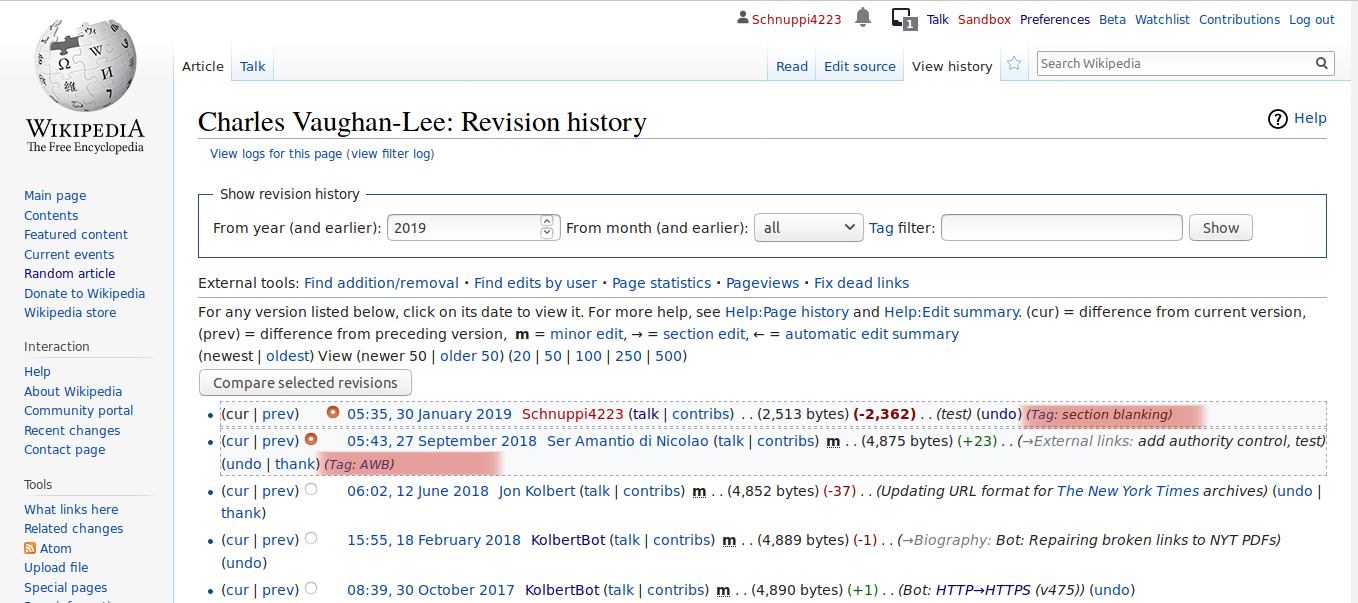
\includegraphics[width=0.9\columnwidth]{figures/screenshots-filter-trigger/Screenshot-tags-in-revision-history.png}
  \caption{Tagged edits are marked as such in a page's revision history}~\label{fig:tags-in-history}
\end{figure}

\begin{figure}
\centering
  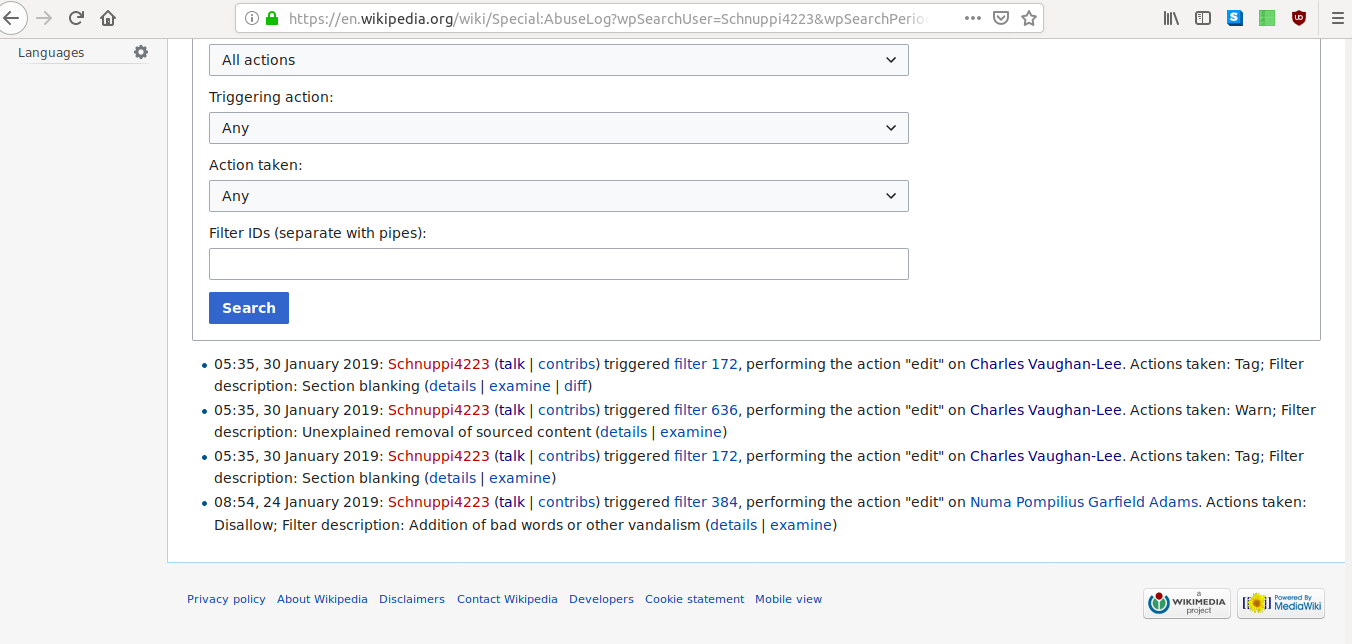
\includegraphics[width=0.9\columnwidth]{figures/screenshots-filter-trigger/Screenshot-abuse-log.png}
  \caption{Abuse Log showing all filter triggers by User Schnuppi4223}~\label{fig:screenshot-abuse-log}
\end{figure}

If the filter is set to disallow, a specific template is shown to the editor: "An automated filter has identified this edit as potentially unconstructive, so it has been disallowed. If this edit is constructive, please report this error. Disruptive editing may result in a block from editing."
"report this error" links to the FalsePositives page: \url{https://en.wikipedia.org/wiki/Wikipedia:Edit_filter/False_positives}
"block from editing" links to \url{https://en.wikipedia.org/wiki/Wikipedia:Blocking_policy}

The edit is not saved.

\begin{figure}
\centering
  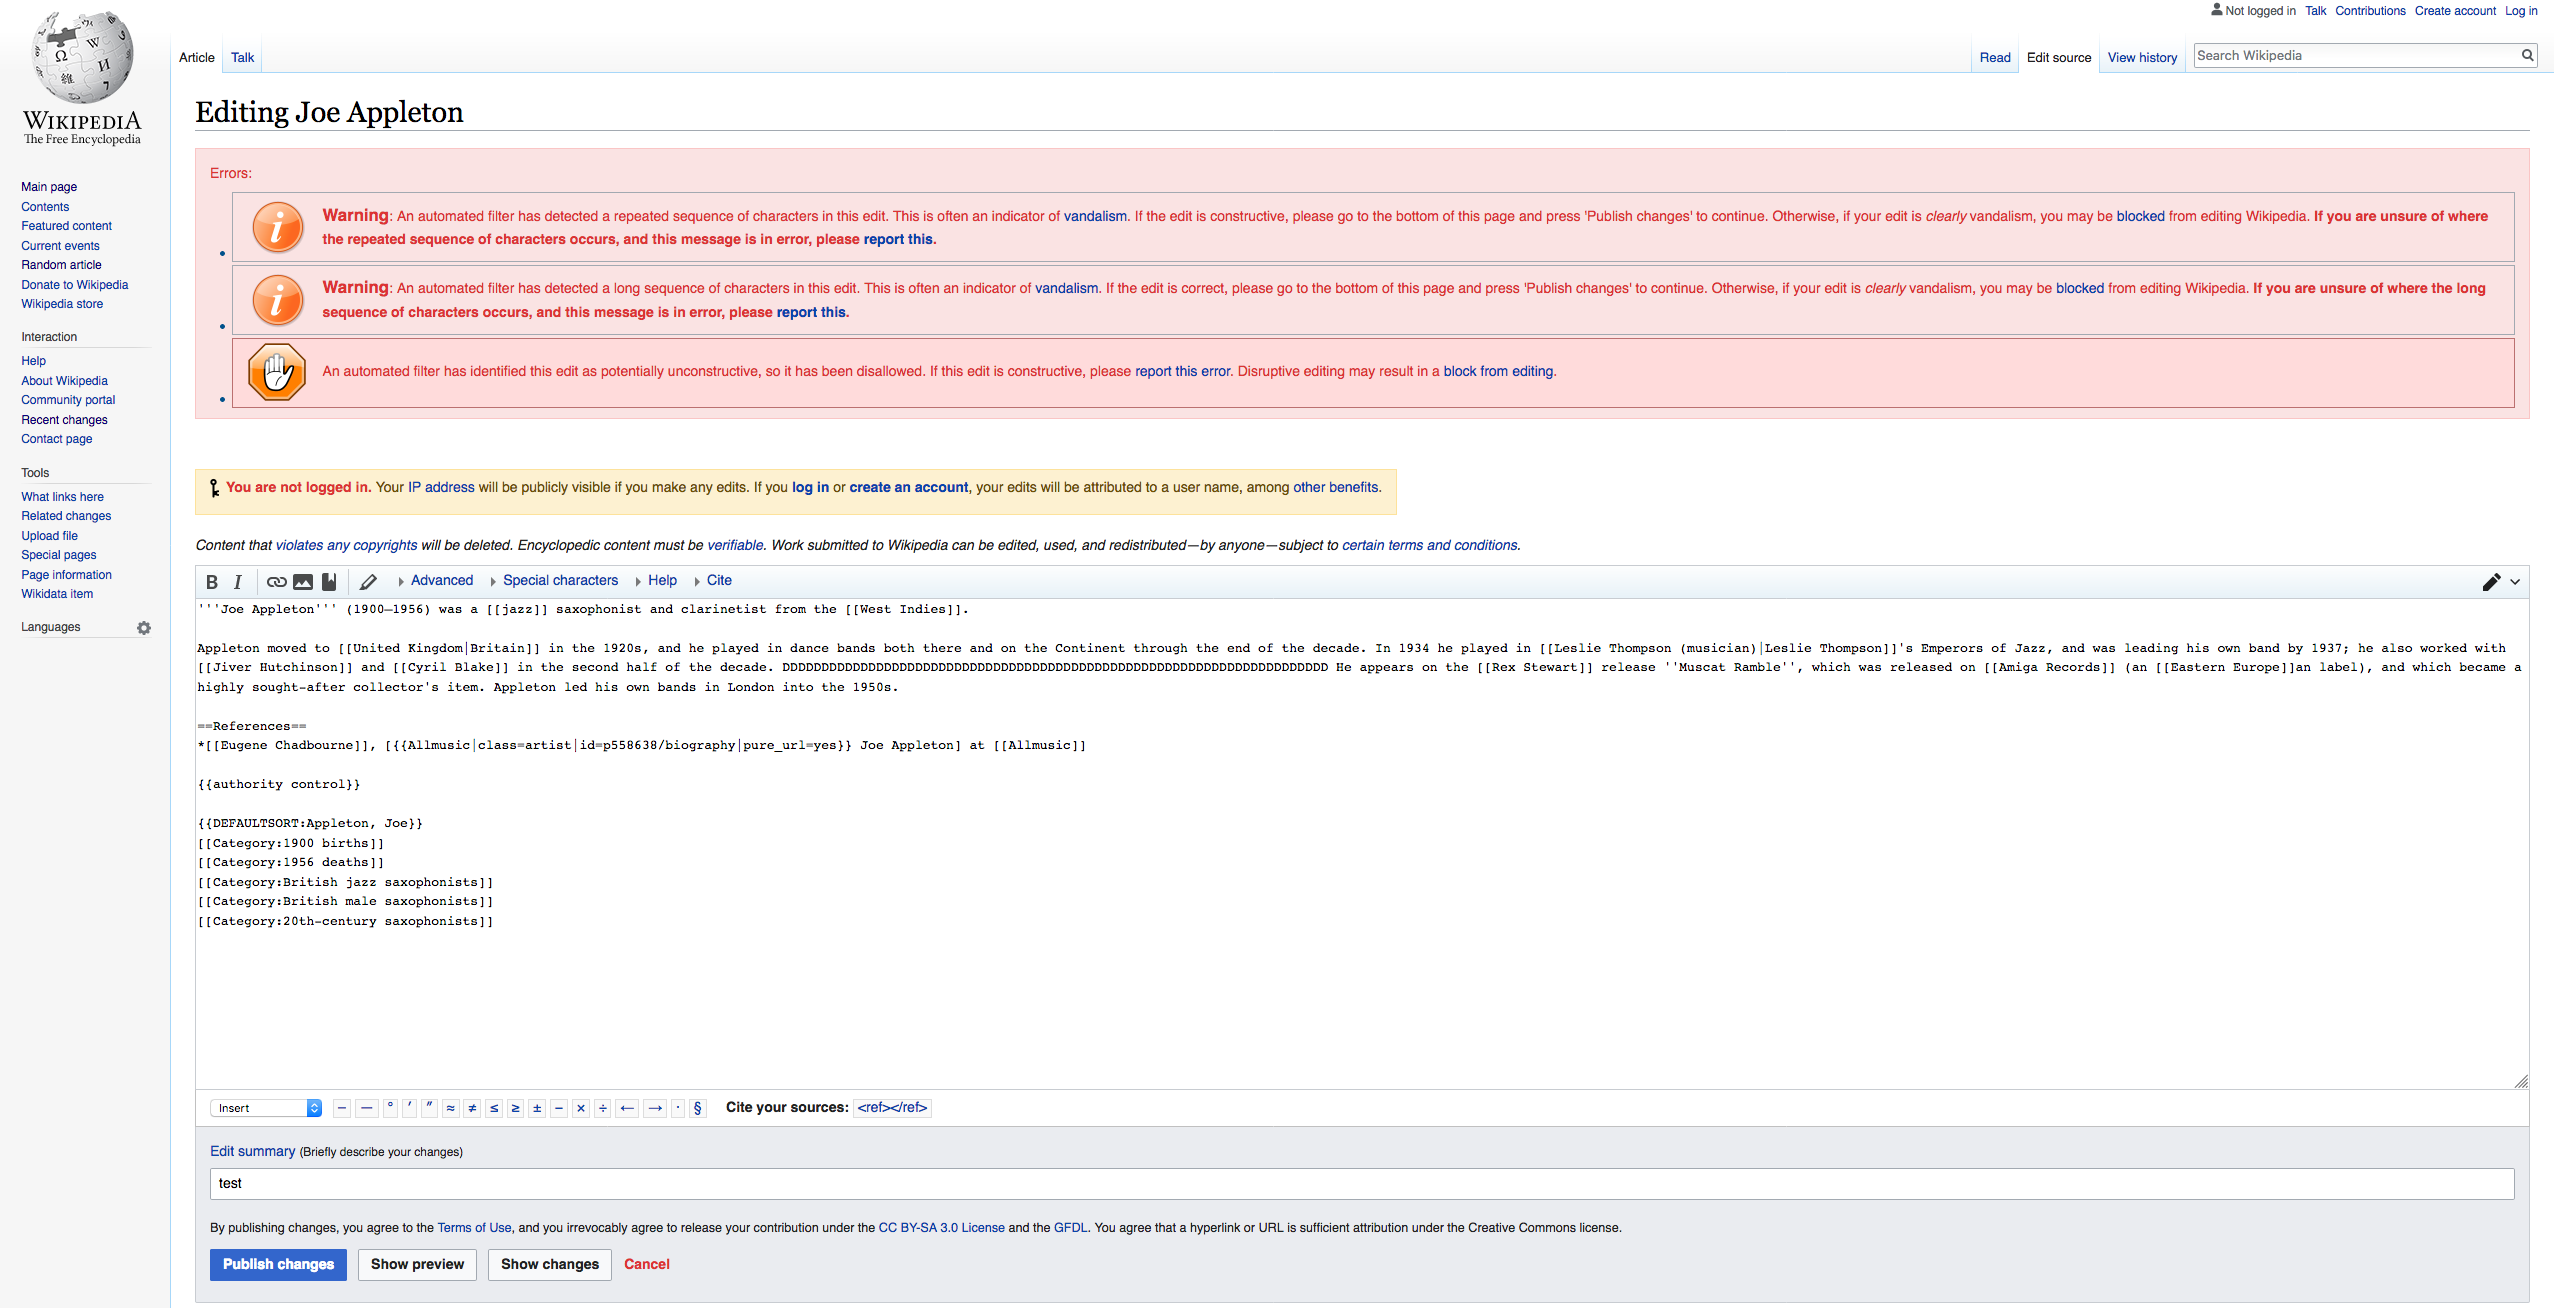
\includegraphics[width=0.9\columnwidth]{figures/screenshots-filter-trigger/Screenshot-trigger-warning-filter.png}
  \caption{Editor gets notified their edit triggered multiple edit filters}~\label{fig:screenshot-warn-disallow}
\end{figure}

\subsection{TOR}
(Interesting side note: editing via TOR is disallowed altogether: "Your IP has been recognised as a TOR exit node. We disallow this to prevent abuse" or similar, check again for wording. Compare: "Users of the Tor anonymity network will show the IP address of a Tor "exit node". Lists of known Tor exit nodes are available from the Tor Project's Tor Bulk Exit List exporting tool." \url{https://en.wikipedia.org/wiki/Wikipedia:Vandalism})


%************************************************************************

\section{Descriptive overview of Edit Filters on the English Wikipedia}

\textbf{Interesting questions}
\begin{itemize}
    \item how many filters are there (were there over the years): 954 filters (stand: 06.01.2019); TODO: historically?; This includes deleted filters
    \item what do the most active filters do?: see~\ref{tab:most-active-actions}
    \item get a sense of what gets filtered (more qualitative): TODO: refine after sorting through manual categories; preliminary: vandalism; unintentional suboptimal behavior from new users who don't know better ("good faith edits") such as blanking an article/section; creating an article without categories; adding larger texts without references; large unwikified new article (180); or from users who are too lazy (to write proper edit summaries; editing behaviours and styles not suitable for an encyclopedia (poor grammar/not commiting to orthography norms; use of emoticons and !; ascii art?); "unexplained removal of sourced content" (636) may be an attempt to silence a view point the editor doesn't like; self-promotion(adding unreferenced material to BLP; "users creating autobiographies" 148;); harassment; sockpuppetry; potential copyright violations; that's more or less it actually. There's a third bigger cluster of maintenance stuff, such as tracking bugs or other problems, trying to sort through bot edits and such. For further details see the jupyter notebook.
        Interestingly, there was a guideline somewhere stating that no trivial behaviour should trip filters (e.g. starting every paragraph with a small letter;) I actually think, a bot fixing this would be more appropriate.
    \item has the willingness of the community to use filters increased over time?: looking at aggregated values of number of triggered filters per year, the answer is rather it's quite constant; TODO: plot it at a finer granularity
        when aggregating filter triggers per month, one notices that there's an overall slight upward tendency.
        Also, there is a dip in the middle of 2014 and a notable peak at the beginning of 2016, that should be investigated further.
    \item how often were (which) filters triggered: see \url{filter-lists/20190106115600_filters-sorted-by-hits.csv} and~\ref{tab:most-active-actions}; see also jupyter notebook for aggregated hitcounts over tagged categories
    \item percentage of triggered filters/all edits; break down triggered filters according to typology: TODO still need the complete abuse\_filter\_log table!; and probably further dumps in order to know total number of edits
    \item percentage filters of different types over the years: according to actions (I need a complete abuse\_filter\_log table for this!); according to self-assigned tags %TODO plot!
    \item what gets classified as vandalism? has this changed over time? TODO: (look at words and patterns triggered by the vandalism filters; read vandalism policy page); pay special attention to filters labeled as vandalism by the edit filter editors (i.e. in the public description) vs these I labeled as vandalism
\end{itemize}

\textbf{Questions on abuse\_filter table}
\begin{itemize}
    \item how many filters are there altogether
    \item how many are enabled/disabled?
    \item how many hidden filters? how many of them are enabled
    \item how many are marked as deleted? (how many of them are hidden?)
    \item how many global? (what does global mean?)
    \item how many throttled? (what does this mean?)
    \item how many currently trigger which action (disallow, warn, throttle, tag, ..)?
    \item explore timestamp (I think it means "last modified"): have a lot of filters been modified recently?
    \item what are the values in the "group" column? what do they mean?
    \item which are the most frequently triggered filters of all time?
    \item is it new filters that get triggered most frequently? or are there also very active old ones?
    \item how many different edit filter editors are there (af\_user)?
    \item categorise filters according to which name spaces they apply to; pay special attention to edits in user/talks name spaces (may be indication of filtering harassment)
\end{itemize}

\textbf{Questions on abuse\_filter\_log table}
\begin{itemize}
    \item how often were filters with different actions triggered? (afl\_actions)
    \item what types of users trigger the filters (IPs? registered?) : IPs: 16,489,266, logged in users: 6,984,897 (Stand 15.03.2019);
    \item on what articles filters get triggered most frequently (afl\_title)
    \item what types of user actions trigger filters most frequently? (afl\_action) (edit, delete, createaccount, move, upload, autocreateaccount, stashupload)
    \item in which namespaces get filters triggered most frequently?
\end{itemize}

\textbf{Questions on abuse\_filter\_action table}
\begin{itemize}
    \item how many filters trigger any particular action (at the moment)?
    \item how many different parameters are there (i.e. tags when tagging, or templates to show upon a warning)?
\end{itemize}

\textbf{Number of unique filters that were triggered each year since 2009:}
owing to quarries we have all the filters that were triggered from the filter log per year, from 2009 (when filters were first introduced/the MediaWiki extension was enabled) till end of 2018 with their corresponding number of times being triggered:
\begin{table}
  \centering
  \begin{tabular}{l r }
    % \toprule
    Year & Num of distinct filters \\
    \hline
    2009 & 220 \\
    2010 & 163 \\
    2011 & 161 \\
    2012 & 170 \\
    2013 & 178 \\
    2014 & 154 \\
    2015 & 200 \\
    2016 & 204 \\
    2017 & 231 \\
    2018 & 254 \\
    % \bottomrule
  \end{tabular}
  \caption{Count of distinct filters that got triggered each year}~\label{tab:active-filters-count}
\end{table}

data is still not enough for us to talk about a tendency towards introducing more filters (after the initial dip)


\textbf{Most frequently triggered filters for each year:}
10 most active filters per year:
\begin{table}
  \centering
  \begin{tabular}{r r }
    % \toprule
    Filter ID & Hitcount \\
    \hline
    135 & 175455 \\
    30 & 160302 \\
    61 & 147377 \\
    18 & 133640 \\
    3 & 95916 \\
    172 & 89710 \\
    50 & 88827 \\
    98 & 80434 \\
    65 & 74098 \\
    132 & 68607 \\
    % \bottomrule
  \end{tabular}
  \caption{10 most active filters in 2009}~\label{tab:most-active-2009}
\end{table}

\begin{table}
  \centering
  \begin{tabular}{r r }
    % \toprule
    Filter ID & Hitcount \\
    \hline
    61 & 245179 \\
    135 & 242018 \\
    172 & 148053 \\
    30 & 119226 \\
    225 & 109912 \\
    3 & 105376 \\
    50 & 101542 \\
    132 & 78633 \\
    189 & 74528 \\
    98 & 54805 \\
    % \bottomrule
  \end{tabular}
  \caption{10 most active filters in 2010}~\label{tab:most-active-2010}
\end{table}

\begin{table}
  \centering
  \begin{tabular}{r r }
    % \toprule
    Filter ID & Hitcount \\
    \hline
    61 & 218493 \\
    135 & 185304 \\
    172 & 119532 \\
    402 & 109347 \\
    30 & 89151 \\
    3 & 75761 \\
    384 & 71911 \\
    225 & 68318 \\
    50 & 67425 \\
    432 & 66480 \\
    % \bottomrule
  \end{tabular}
  \caption{10 most active filters in 2011}~\label{tab:most-active-2011}
\end{table}

\begin{table}
  \centering
  \begin{tabular}{r r }
    % \toprule
    Filter ID & Hitcount \\
    \hline
    135 & 173830 \\
    384 & 144202 \\
    432 & 126156 \\
    172 & 105082 \\
    30 & 93718 \\
    3 & 90724 \\
    380 & 67814 \\
    351 & 59226 \\
    279 & 58853 \\
    225 & 58352 \\
    % \bottomrule
  \end{tabular}
  \caption{10 most active filters in 2012}~\label{tab:most-active-2012}
\end{table}

\begin{table}
  \centering
  \begin{tabular}{r r }
    % \toprule
    Filter ID & Hitcount \\
    \hline
    135 & 133309 \\
    384 & 129807 \\
    432 & 94017 \\
    172 & 92871 \\
    30 & 85722 \\
    279 & 76738 \\
    3 & 70067 \\
    380 & 58668 \\
    491 & 55454 \\
    225 & 48390 \\
    % \bottomrule
  \end{tabular}
  \caption{10 most active filters in 2013}~\label{tab:most-active-2013}
\end{table}

\begin{table}
  \centering
  \begin{tabular}{r r }
    % \toprule
    Filter ID & Hitcount \\
    \hline
    384 & 111570 \\
    135 & 111173 \\
    279 & 97204 \\
    172 & 82042 \\
    432 & 75839 \\
    30 & 62495 \\
    3 & 60656 \\
    636 & 52639 \\
    231 & 39693 \\
    380 & 39624 \\
    % \bottomrule
  \end{tabular}
  \caption{10 most active filters in 2014}~\label{tab:most-active-2014}
\end{table}

\begin{table}
  \centering
  \begin{tabular}{r r }
    % \toprule
    Filter ID & Hitcount \\
    \hline
    650 & 226460 \\
    61 & 196986 \\
    636 & 191320 \\
    527 & 189911 \\
    633 & 162319 \\
    384 & 141534 \\
    279 & 110137 \\
    135 & 99057 \\
    686 & 95356 \\
    172 & 82874 \\
    % \bottomrule
  \end{tabular}
  \caption{10 most active filters in 2015}~\label{tab:most-active-2015}
\end{table}

\begin{table}
  \centering
  \begin{tabular}{r r }
    % \toprule
    Filter ID & Hitcount \\
    \hline
    527 & 437099 \\
    61 & 274945 \\
    650 & 229083 \\
    633 & 218696 \\
    636 & 179948 \\
    384 & 179871 \\
    279 & 106699 \\
    135 & 95131 \\
    172 & 79843 \\
    30 & 68968 \\
    % \bottomrule
  \end{tabular}
  \caption{10 most active filters in 2016}~\label{tab:most-active-2016}
\end{table}

\begin{table}
  \centering
  \begin{tabular}{r r }
    % \toprule
    Filter ID & Hitcount \\
    \hline
    61 & 250394 \\
    633 & 218146 \\
    384 & 200748 \\
    527 & 192441 \\
    636 & 156409 \\
    650 & 151604 \\
    135 & 80056 \\
    172 & 70837 \\
    712 & 59537 \\
    833 & 58133 \\
    % \bottomrule
  \end{tabular}
  \caption{10 most active filters in 2017}~\label{tab:most-active-2017}
\end{table}

\begin{table}
  \centering
  \begin{tabular}{r r }
    % \toprule
    Filter ID & Hitcount \\
    \hline
    527 & 358210 \\
    61 & 234867 \\
    633 & 201400 \\
    384 & 177543 \\
    833 & 161030 \\
    636 & 144674 \\
    650 & 79381 \\
    135 & 75348 \\
    686 & 70550 \\
    172 & 64266 \\
    % \bottomrule
  \end{tabular}
  \caption{10 most active filters in 2018}~\label{tab:most-active-2018}
\end{table}

\textbf{what do the most active filters do?}

\begin{table*}
  \centering
    \begin{tabular}{r p{10cm} p{5cm} }
    % \toprule
    Filter ID & Publicly available description & Actions \\
    \hline
      135 & repeating characters & tag, warn \\
      30 & "large deletion from article by new editors" & tag, warn \\
      61 & "new user removing references" ("new user" is handled by "!("confirmed" in user\_groups)") & tag \\
      18 & "test type edits from clicking on edit bar" (people don't replace Example texts when click-editing) & deleted in Feb 2012 \\
      3 & "new user blanking articles" & tag, warn \\
      172 & "section blanking" & tag \\
      50 & "shouting" (contribution consists of all caps, numbers and punctuation) & tag, warn \\
      98 & "creating very short new article" & tag \\
      65 & "excessive whitespace" (note: "associated with ascii art and some types of vandalism") & deleted in Jan 2010 \\
      132 & "removal of all categories" & tag, warn \\
      225 & "vandalism in all caps" (difference to 50? seems to be swear words, but shouldn't they be catched by 50 anyway?) & disallow \\
      189 & "BLP vandalism or libel" & tag \\
      402 & "new article without references" & deleted in Apr 2013, before that disabled with comment "disabling, no real use" \\
      384 & "addition of bad words or other vandalism" (seems to be a blacklist) & disallow \\
      432 & "starting new line with lower case letters" & tag, warn //I recall there was a rule of thumb recommending not to user filters for style things? although that's not really style, but rather wrong grammar.. \\
      380 & hidden; public comment "multiple obscenities" & disallow \\
      351 & "text added after categories and interwiki" & tag, warn \\
      279 & "repeated attempts to vandalise" & tag, throttle (triggered when someone hits "edit" repeatedly in a short ammount of time) \\
      491 & "edits ending with emoticons or !" & tag, warn \\
      636 & "unexplained removal of sourced content" & warn (that, together with 634 and 635 refutes my theory that warn always goes together with tag) \\
      231 & "long string of characters containing no spaces" (that's surely english though^^) & tag, warn \\
      650 & "creation of a new article without any categories" & (log only) \\
      527 & hidden; public comments "T34234: log/throttle possible sleeper account creations" & throttle \\
      633 & "possible canned edit summary" (apparently pre-filled on mobile though) & tag \\
      686 & "IP adding possible unreferenced material to BLP" (BLP= biography of living people? I thought, it was forbidden to edit them without a registered account) & (log only) \\
      712 & "possibly changing date of birth in infobox" ("possibly"? and I thought infoboxes were pre-generated from wikidata?) & (log only) \\
      833 & "newer user possibly adding a unreferenced or improperly referenced material" & (log only) \\
  \end{tabular}
  \caption{What do most active filters do?}~\label{tab:most-active-actions}
\end{table*}

A lot of filters are disabled/deleted bc:
* they hit too many false positives
* they were implemented to target specific incidents and these vandalism attempts stopped
* they were tested and merged into other filters
* there were too few hits and the conditions were too expensive

Multiple filters have the comment "let's see whether this hits something", which brings us to the conclusion that edit filter editors have the right and do implement filters they consider necessary


\subsection{Types of edit filters}

We can sort filters into categories along various criteria.

\subsubsection{Public and Hidden Filters}

The first noticeable typology is along the line public/private filters.

It is calling attention that nearly 2/3 of all edit filters are not viewable by the general public.

The guidelines call for hiding filters ``only where necessary, such as in long-term abuse cases where the targeted user(s) could review a public filter and use that knowledge to circumvent it.''~\cite{Wikipedia:EditFilter}.
Further, they suggest caution in filter naming and giving just simple description of the overall disruptive behaviour rather than naming specificuser that is causing the disruptions.
(The later is not always complied with, there are indeed filters named after the accounts causing a disruption.)

Only edit filter editors (who have the \emph{abusefilter-modify} permission) and editors with the \emph{abusefilter-view-private} permission can view hidden filters.
The later is given to edit filter helpers - editors interested in helping with edit filters who still do not meet certain criteria in order to be granted the full \emph{abusefilter-modify} permission, editors working with edit filters on other wikis interested in learning from the filter system on English Wikipedia, and Sockpuppet investigation clerks~\cite{Wikipedia:EditFilterHelper}.
As of March 17, 2019, there are 16 edit filter helpers on EN Wikipedia~\footnote{\url{https://en.wikipedia.org/wiki/Special:ListUsers/abusefilter-helper}}.
Also, all administrators are able to view hidden filters.

There is also a designated mailing list for discussing these: wikipedia-en-editfilters@lists.wikimedia.org.
It is specifically indicated that this is the communication channel to be used when dealing with harassment (by means of edit filters)~\cite{Wikipedia:EditFilter}.
It is signaled, that the mailing list is meant for sensitive cases only and all general discussions should be held on-wiki~\cite{Wikipedia:EditFilter}.

\begin{comment}
\url{https://en.wikipedia.org/wiki/Wikipedia:Edit_filter}
"Non-admins in good standing who wish to review a proposed but hidden filter may message the mailing list for details."
// what is "good standing"?
// what are the arguments for hiding a filter? --> particularly obnoctious vandals can see how their edits are being filtered and circumvent them; security through obscurity
// are users still informed if their edit triggers a hidden filter? - most certainly; the warnings logic has nothing to do with whether the filter is hidden or not

"For all filters, including those hidden from public view, a brief description of what the rule targets is displayed in the log, the list of active filters, and in any error messages generated by the filter. " //yeah, well, that's the public comment, aka name of the filter

"Be careful not to test sensitive parts of private filters in a public test filter (such as Filter 1): use a private test filter (for example Filter 2) if testing is required."

\end{comment}

\subsection{Types of edit filters: Manual Classification}

Apart from filter typologies that can be derived directly from the DB schema (available fields/existing features), we propose a manual classification of the types of edits edit filters found on the EN Wikipedia target (there are edit filters with different purposes).

Based on the GT methodology, we scrutinised all filters, with their patterns, comments and actions.
We found 3 big clusters of filters that we labeled ``vandalism'', ``good faith'' and ``maintenance''.
It was not always a straightforward desicion to determine what type of edits a certain filter is targeting.
This was of course, particularly challenging for private filters where only the public comment (name) of the filter was there to guide us.
On the other hand, guidelines state up-front that filters should be hidden only in cases of particularly persistent vandalism, in so far it is probably safe to establish that all hidden filters target some type of vandalism.
However, the classification was difficult for public filters as well, since oftentimes what makes the difference between a good-faith and a vandalism edit is not the content of the edit but the intention of the editor.
While there are cases of juvenile vandalism (putting random swear words in articles) or characters repetiton vandalism which are pretty obvious, that is not the case for sections or articles blanking for example.
In such ambiguous cases, we can be guided by the action the filter triggers (if it is ``disallow'' the filter is most probably targeting vandalism).
At the end, we labeled most ambiguous cases with both ``vandalism'' and ``good faith''.

In the subsections that follow we discuss the salient properties of each manually labeled category.

%TODO: develop and include memos
\subsubsection{Vandalism}

\subsubsection{Good Faith}

\subsubsection{Maintenance}


Following filter categories have been identified (sometimes, a filter was labeled with more than one tag):
%TODO make a diagramm with these
- Vandalism
  - hoaxing
  - silly vandalism (e.g. repeating characters, inserting swear words)
  - spam
  - sockpuppetry
  - long term abuse // there seems to be separate documentation for this, see notes;
  - harassment/personal attacks
    - doxxing
    - impersonation
  - trolling
  - copyright violation

  Labeled along the vandalism typology (check above)
  - link vandalism
  - abuse of tags
  - username vandalism
  - image vandalism
  - avoidant vandalism
  - talk page vandalism
  - page move vandalism
  - template vandalism
  - vandalbots

  Kind of similar:
  - seo
  - stockbroker vandalism
  - biased pov
  - self promotion
  - conflict of interest

Inbetween
- edit warring
- political controversy
- politically/religiously motivated hate

- Good faith
  - bad style ("unencyclopedic edits" e.g. citing a blog or mentioning a hypothetical future album release)
  - lazyness


- Maintenance
  - bugs
  - wiki policy (compliance therewith)
  - test filters

\section{Limitations}

This work presents a first attempt at analysing Wikipedia's edit filter system.
It has several limitations (we could think of).
First, it focuses on English Wikipedia only.
We are convinced that there are valuable lessons to be learnt (about the communities, usefulness of filters, ..) from comparing edit filter use across different language versions.
Second, unfortunately, including an ethnographic analysis was not possible.
This is partially due to the fact that we employ a computer science perspective on the question and partially due to limited time.
Third, the manual filter classification was undertaken by one person only, so biases of this person have certainly shaped the labels.

\section{Discussion}

* why get certain filters (and not others?)
* do filters solve effectively the task they were conjured up to life to fulfil?
* what kinds of biases/problems are there?
* who is allowed to edit edit filters?

Alternative approaches to community management:
compare with Surviving the Eternal September paper~\cite{KieMonHill2016}
"importance of strong
systems of norm enforcement made possible by leadership,
community engagement, and technology."

"emphasizing decentralized moderation" //all community members help enforce the norms
"ensuring enough leadership capacity is available
when an influx of newcomers is anticipated."
"Designers may
benefit by focusing on tools to let existing leaders bring others
on board and help them clearly communicate norms."
"designers should support an ecosystem of accessible and ap-
propriate moderator tools."


\subsection{The bigger picture: Upload filters}

The planned introduction of upload filters by the EU copyright reform is seen critically by Wikimedia Germany:
\begin{figure}
\centering
  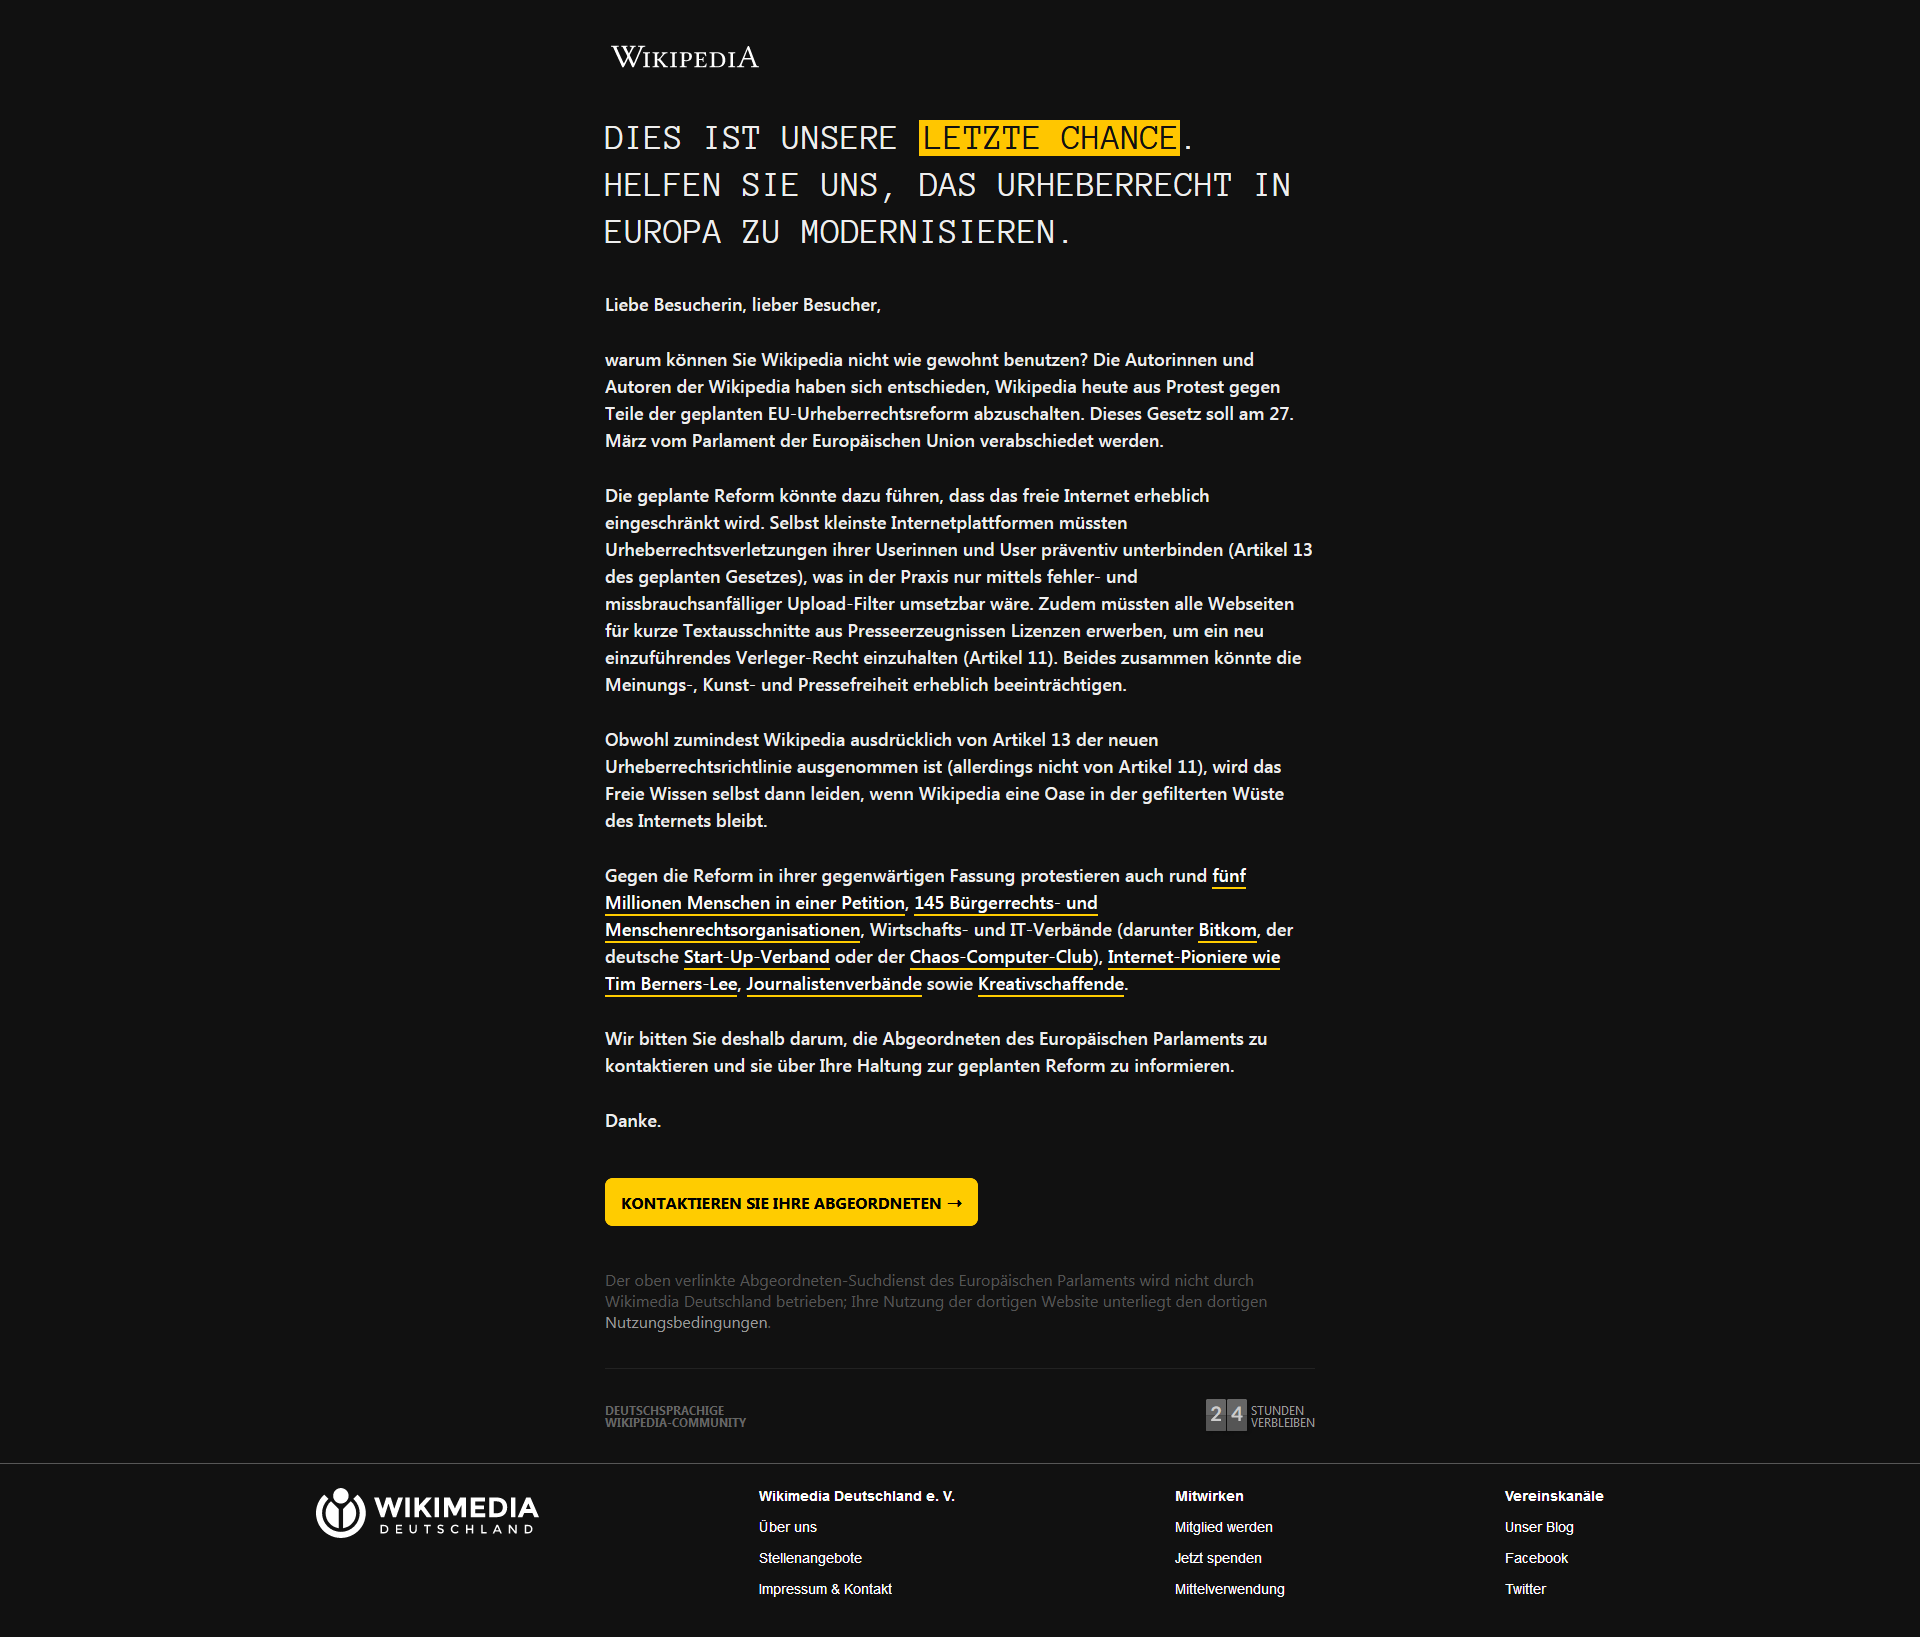
\includegraphics[width=0.9\columnwidth]{figures/Blackout_of_wikipedia.de_by_Wikimedia_Deutschland_-_March_2019.png}
  \caption{Blackout of wikipedia.de by Wikimedia Deutschland}~\label{fig:blackout-upload-filters}
\end{figure}

via
\url{https://de.wikipedia.org/wiki/Abschaltung_der_deutschsprachigen_Wikipedia_am_21._M%C3%A4rz_2019#/media/File:Blackout_of_wikipedia.de_by_Wikimedia_Deutschland_-_March_2019.png}

see also
\url{https://wikimediafoundation.org/2019/03/20/four-wikipedias-to-black-out-over-eu-copyright-directive/}
"Volunteer editor communities in four language Wikipedias—German, Czech, Danish, and Slovak—have decided to black out the sites on 21 March in opposition to the current version of the proposed EU Copyright Directive.

Those language editions of Wikipedia will redirect all visitors to a banner about the directive, blocking access to content on Wikipedia for 24 hours. "
"These independent language communities decided to black out in the same way most decisions are made on Wikipedia—through discussion and consensus, "

and
\url{https://wikimediafoundation.org/2019/02/28/we-do-not-support-the-eu-copyright-directive-in-its-current-form-heres-why-you-shouldnt-either/}

timeline
\url{https://edri.org/upload-filters-status-of-the-copyright-discussions-and-next-steps/}

\url{https://en.wikipedia.org/wiki/Directive_on_Copyright_in_the_Digital_Single_Market#Positions}

\subsection{Directions for further studies}
<insert long list of interesting questions here>

\section{Conclusion}

It is important that you write for the SIGCHI audience. Please read
previous years' proceedings to understand the writing style and
conventions that successful authors have used. It is particularly
important that you state clearly what you have done, not merely what
you plan to do, and explain how your work is different from previously
published work, i.e., the unique contribution that your work makes to
the field. Please consider what the reader will learn from your
submission, and how they will find your work useful. If you write with
these questions in mind, your work is more likely to be successful,
both in being accepted into the conference, and in influencing the
work of our field.

\section{Acknowledgments}

Sample text: We thank all the volunteers, and all publications support
and staff, who wrote and provided helpful comments on previous
versions of this document. Authors 1, 2, and 3 gratefully acknowledge
the grant from NSF (\#1234--2012--ABC). \textit{This whole paragraph is
  just an example.}

% Balancing columns in a ref list is a bit of a pain because you
% either use a hack like flushend or balance, or manually insert
% a column break.  http://www.tex.ac.uk/cgi-bin/texfaq2html?label=balance
% multicols doesn't work because we're already in two-column mode,
% and flushend isn't awesome, so I choose balance.  See this
% for more info: http://cs.brown.edu/system/software/latex/doc/balance.pdf
%
% Note that in a perfect world balance wants to be in the first
% column of the last page.
%
% If balance doesn't work for you, you can remove that and
% hard-code a column break into the bbl file right before you
% submit:
%
% http://stackoverflow.com/questions/2149854/how-to-manually-equalize-columns-
% in-an-ieee-paper-if-using-bibtex
%
% Or, just remove \balance and give up on balancing the last page.
%
\balance{}

% BALANCE COLUMNS
\balance{}

% REFERENCES FORMAT
% References must be the same font size as other body text.
\bibliographystyle{SIGCHI-Reference-Format}
\bibliography{literature}

\end{document}

%%% Local Variables:
%%% mode: latex
%%% TeX-master: t
%%% End:
